\section{Arquitectura propuesta}
\begin{frame}
   \frametitle{Arquitectura propuesta}
   \begin{itemize}
   	\item Se centra en la comunicación de la aviónica de un vehículo espacial. 
   	\item Sus componentes primarios son de baja confiabilidad
   	\item Se utiliza el protocolo de comunicación CANae.
   	\item Se propone que la utilización de una filosofía distribuida
   \end{itemize}
\end{frame}

\begin{frame}[c]
		\centering
		\LARGE \textbf{Casos de usos}
\end{frame}

\begin{frame}
	% \centering
	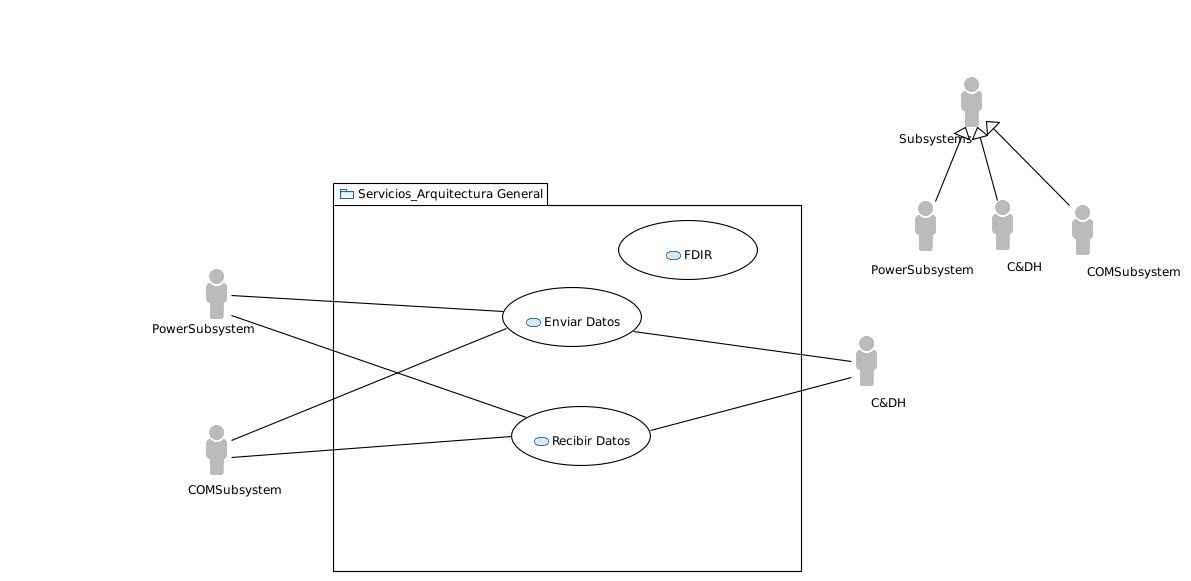
\includegraphics[scale=0.28]{images/Arq_General.JPG}
\end{frame}

\begin{frame}[c]
	\centering
	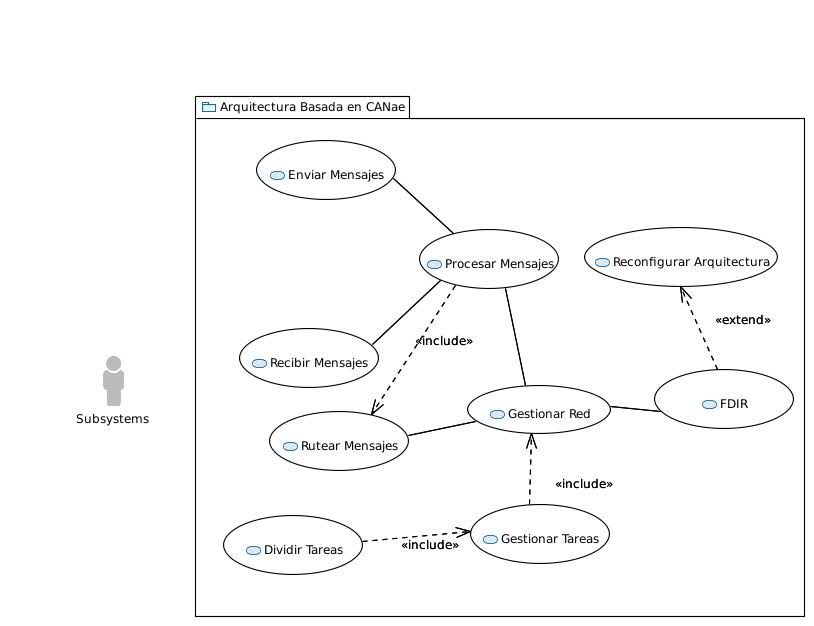
\includegraphics[scale=0.4]{images/Caso_de_Uso_Arquitectura.JPG}
\end{frame}
 
\begin{frame}[c]
	\centering
	\LARGE \textbf{Diseño estructural}
\end{frame}

\begin{frame}
	\frametitle{Diseño estructural}
	\begin{itemize}
		\item La arquitectura presentada rompe con el diseño tradicional de sistemas espaciales
		\item La arquitectura permite conectar una cantidad de N nodos (N < 128). Sus componentes son COTS. 
		\item La red a bajo nivel, deben trabajar bajo normas preestablecidas por algún protocolo preexistente. 
		\item Se aconseja el uso de CANOpen.
		\item Surge la necesidad de desarrollar un Bridge Tolerante a fallas. 
	\end{itemize}
\end{frame}

\begin{frame}[c]
	\centering
	\LARGE \textbf{Configuración de conexión}
\end{frame}

\begin{frame}[c]
	\centering
	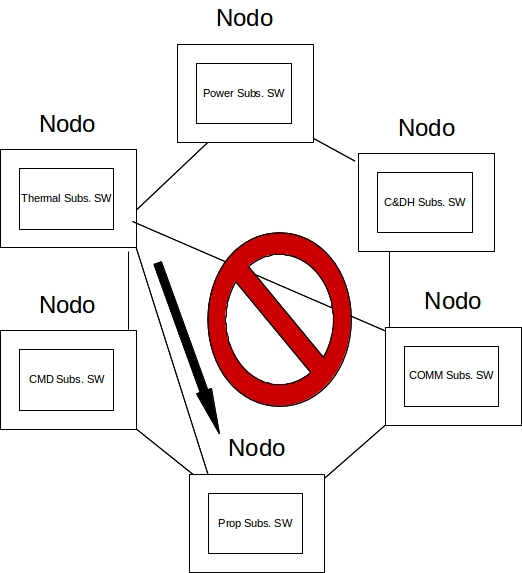
\includegraphics[scale=0.4]{images/Bridge1.jpg}
\end{frame}

\begin{frame}[c]
	\centering
	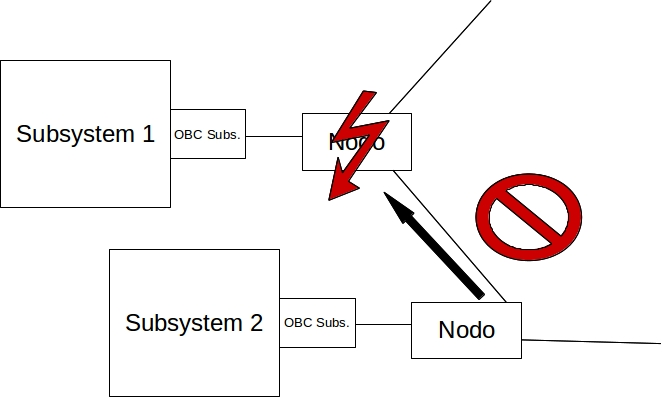
\includegraphics[scale=0.4]{images/Bridge2.jpg}
\end{frame}

\begin{frame}[c]
	\centering
	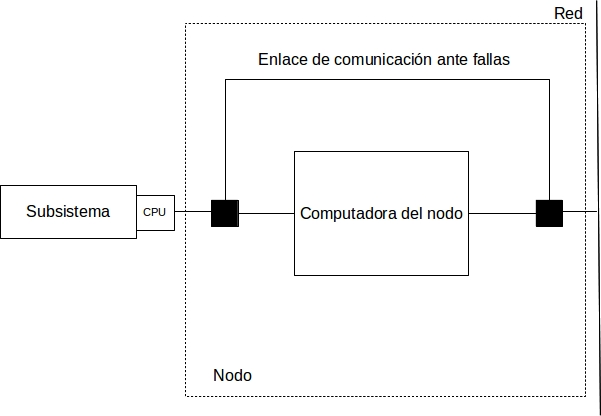
\includegraphics[scale=0.4]{images/com_nodo.jpg}
\end{frame}

\begin{frame}[c]
	\frametitle{Diseño estructural}
	\centering
	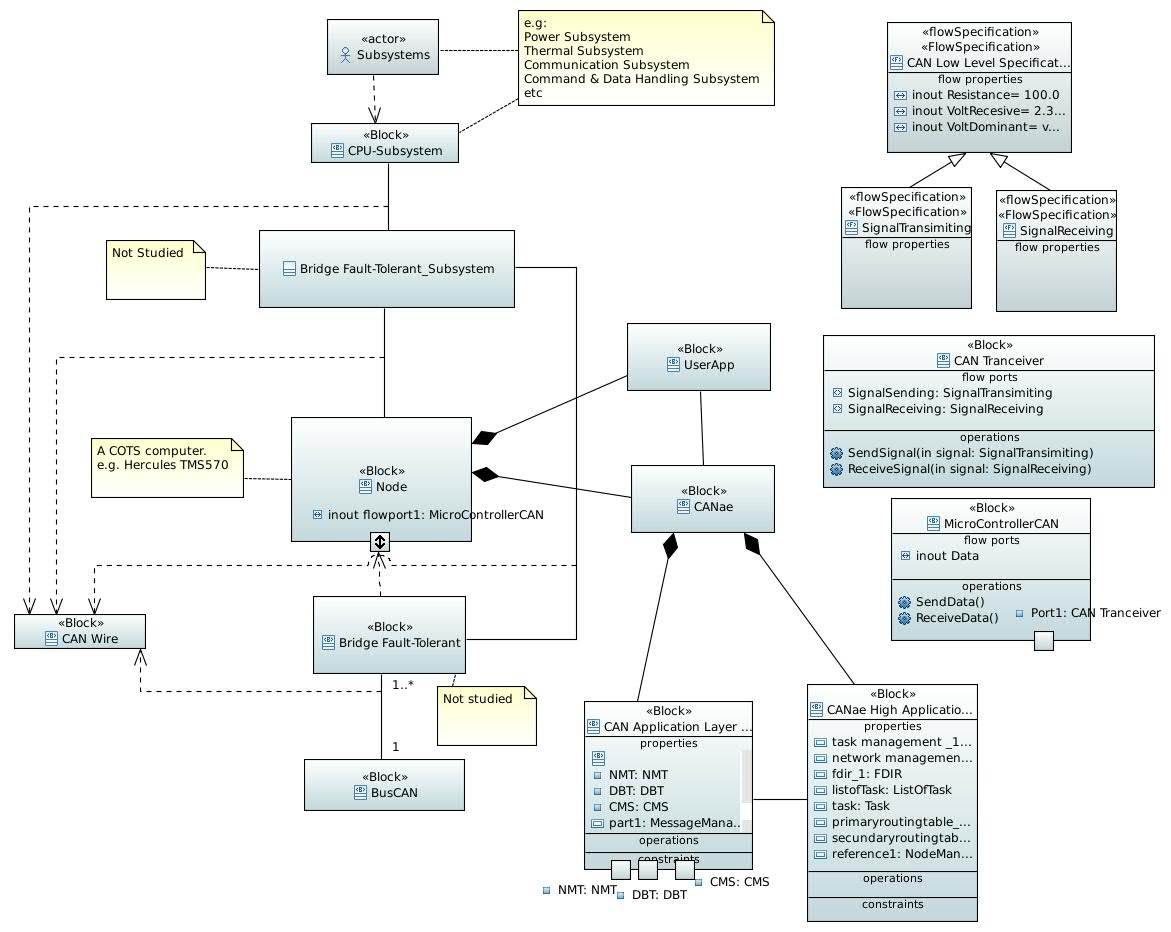
\includegraphics[scale=0.25]{images/ArqCompletaBlockDiagram.JPG}
\end{frame}

\begin{frame}[c]
	\frametitle{Nodo - Internal Block}
	\centering
	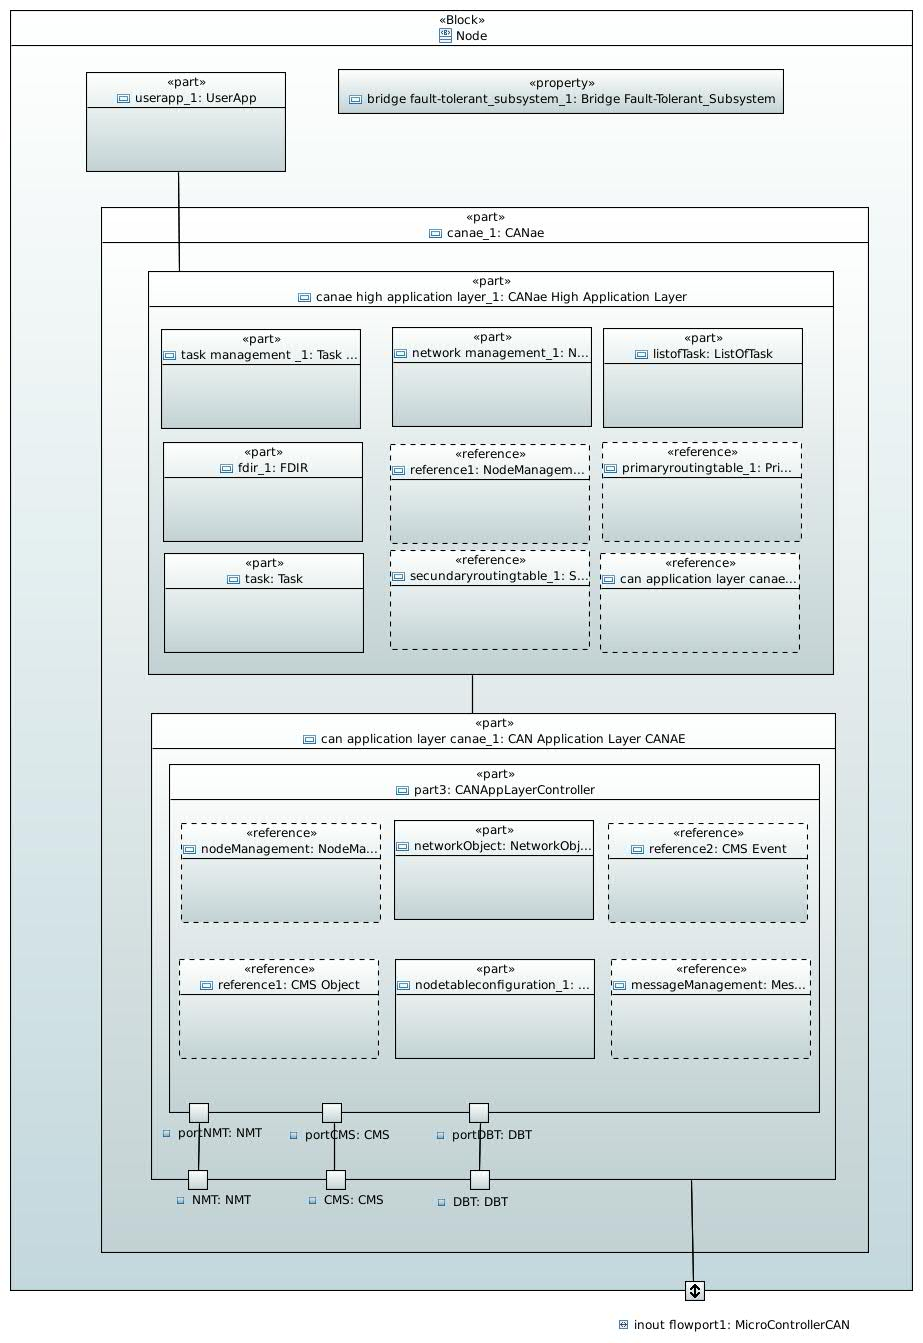
\includegraphics[scale=0.15]{images/NodeInternalDiagram.JPG}
\end{frame}

\begin{frame}[c]
	\centering
	\LARGE \textbf{Máquina de estado}
\end{frame}

\begin{frame}[c]
	\frametitle{Máquina de estado de la arquitectura completa}
	\centering
	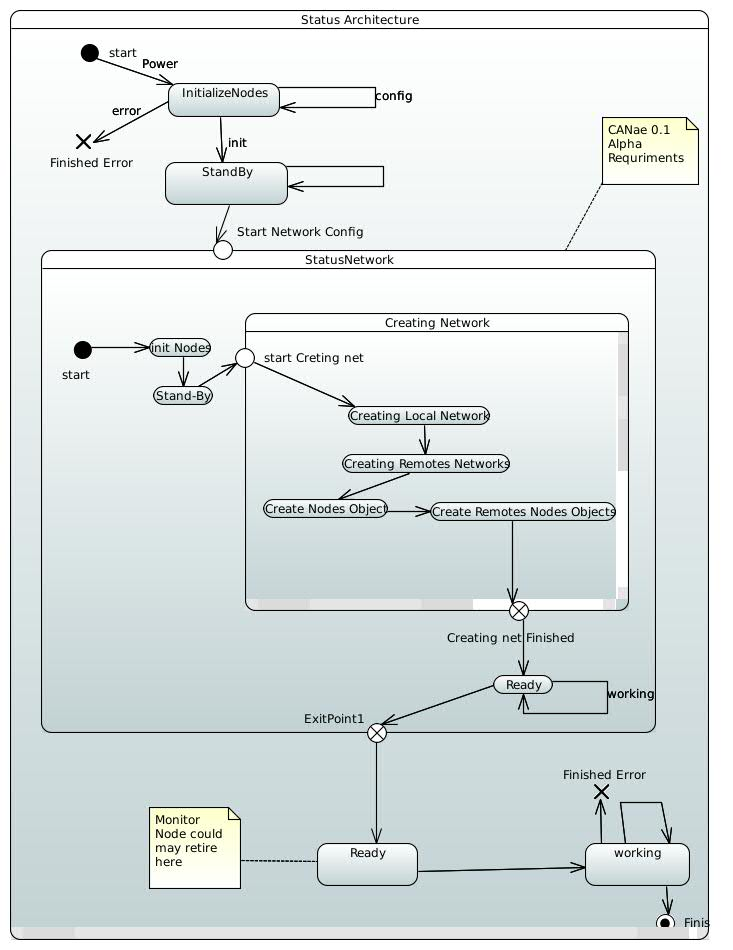
\includegraphics[scale=0.25]{images/StateMachineArqCompleta.JPG}
\end{frame}

\begin{frame}[c]
	\frametitle{Máquina de estado nodos}
	\centering
	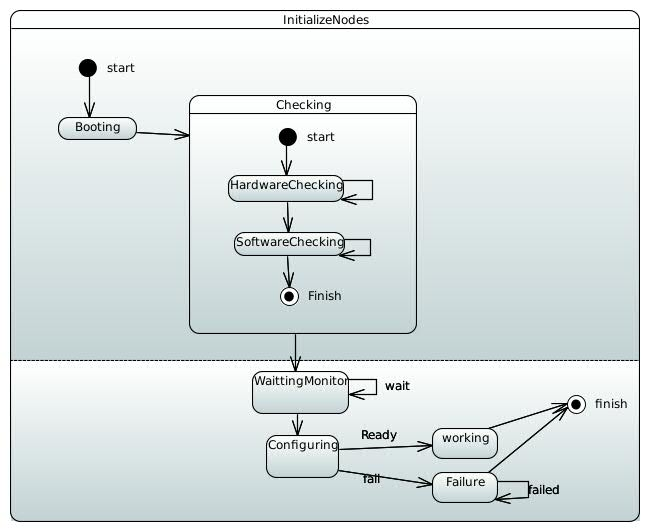
\includegraphics[scale=0.3]{images/InitializeNodes.JPG}
\end{frame}

\begin{frame}[c]
	\centering
	\LARGE \textbf{Diagramas de actividades}
\end{frame}

\begin{frame}[c]
	\frametitle{Inicio de Nodos}
	\centering
	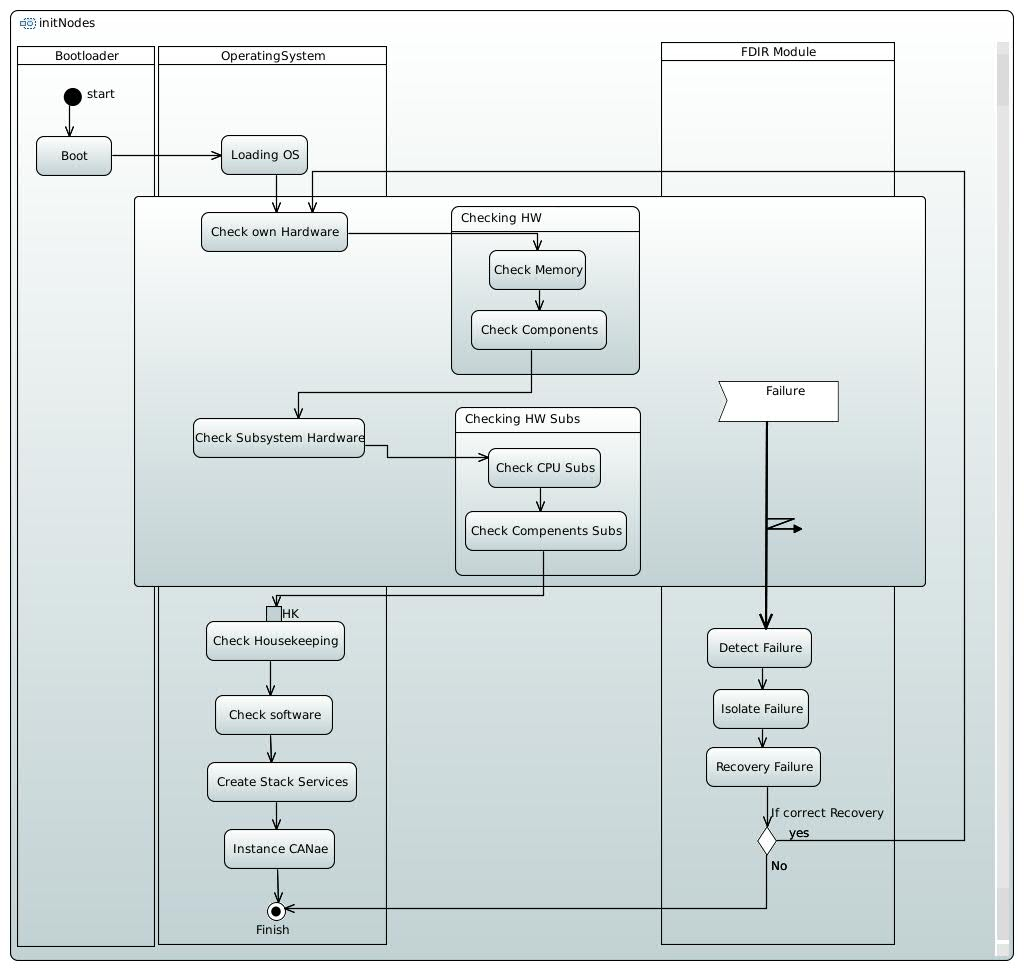
\includegraphics[scale=0.22]{images/initNodes.JPG}
\end{frame}

\begin{frame}[c]
	\frametitle{Nodo Monitor}
	\centering
	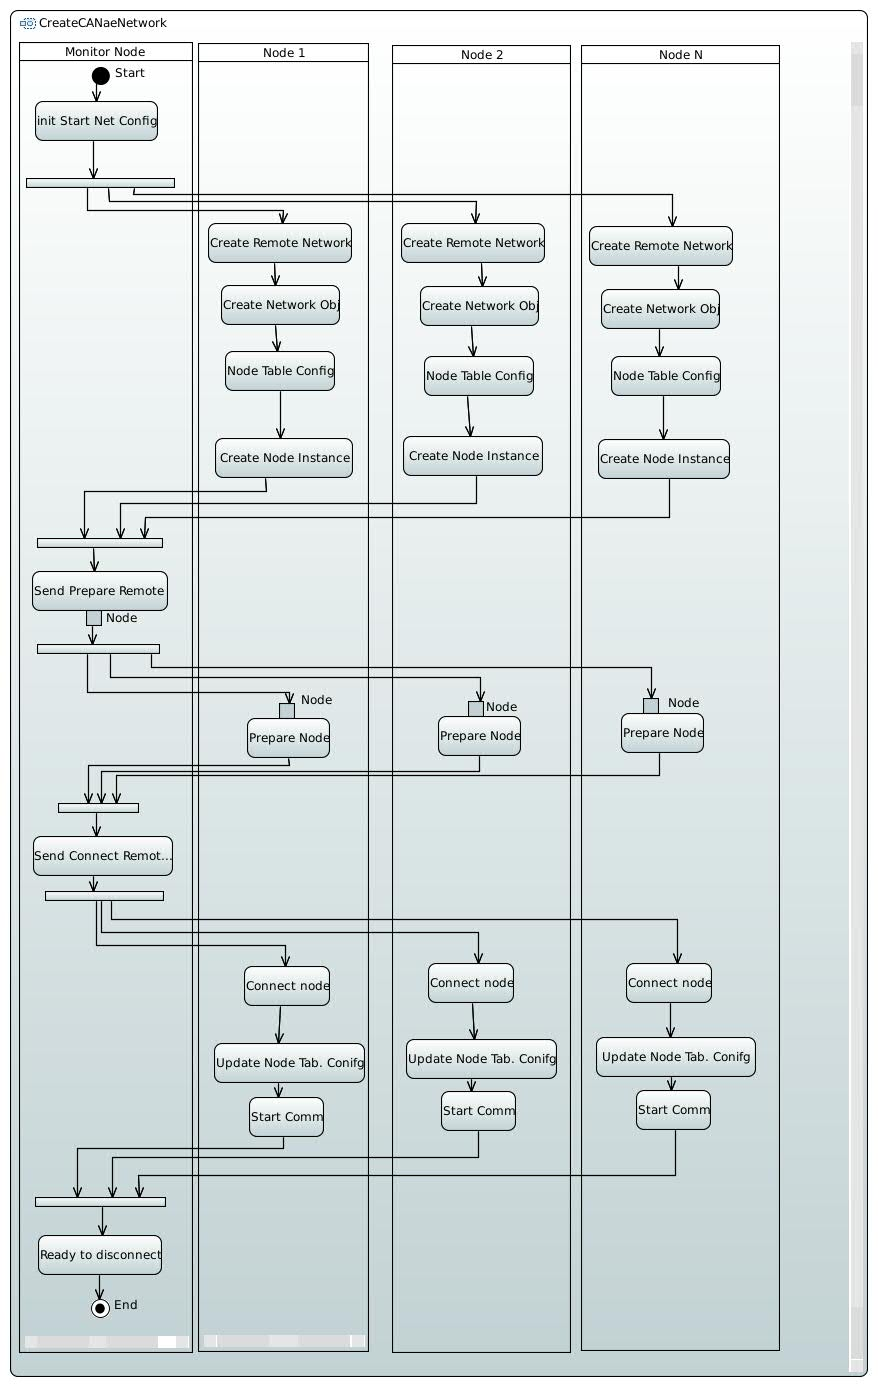
\includegraphics[scale=0.15]{images/NodeMonitor.JPG}
\end{frame}